\subsection{Processo de Desenvolvimento: Nível de Programa e Time}

O gerenciamento da sprint foi feito por quadros Kanban, na qual teremos nove quadros principais. Esses quadros se encontram nos Boards do github, utilizando como base o plugin chamado \href{https://www.zenhub.com/}{Zenhub}. Para instalar é só baixar o plugin e instalar no navegador, a partir daí já conseguirá ver toda organização das issues do projeto a partir da ferramenta. Os quadros são:

\begin{itemize}
  \item \textbf{Epic}: Épicos do software.
  \item \textbf{Features}: \textit{Features} do software.
  \item \textbf{New issues}: Novas histórias de usuário, bug reports ou qualquer tipo de situações de trabalho relacionadas ao desenvolvimento da aplicação que ainda não foram mapeadas, pontuadas ou priorizadas e consequentemente alocadas nos demais quadros.
  \item \textbf{Ice Box}: Issues congeladas por dependência de outras, por alguma necessidade de reavaliação da necessidade ou do esforço necessário para concluí-la, por dependência de funcionalidades externas que não são disponibilizadas pelos mantenedores, por temporária incapacidade da equipe de solucionar determinado problema, etc.
  \item \textbf{Product Backlog}: \textit{Board} para histórias/tarefas ou correções já mapeadas e priorizadas. É importante esclarecer que nesse quadro, a prioridade é definida pela posição da \textit{issue} na \textit{board}, sendo que as posições superiores determinam maior relevância para o projeto.
  \item \textbf{Sprint Backlog}: \textit{Issues} alocadas para os pares na \textit{sprint} corrente ou \textit{bug fixes} de alta prioridade.
  \item \textbf{Review}: Tarefas concluídas que necessitam de revisão para entrarem na aplicação.
  \item \textbf{Done}: Código já revisado que pode ser anexado a aplicação na próxima release.
  \item \textbf{Closed}: \textit{Issues} fechadas já anexado a aplicação.
\end{itemize}

Na figura \ref{fig:desenvolvimento} está definido o processo de desenvolvimento que está no nível de programa e time.

\begin{figure}[h!]
	\centering
  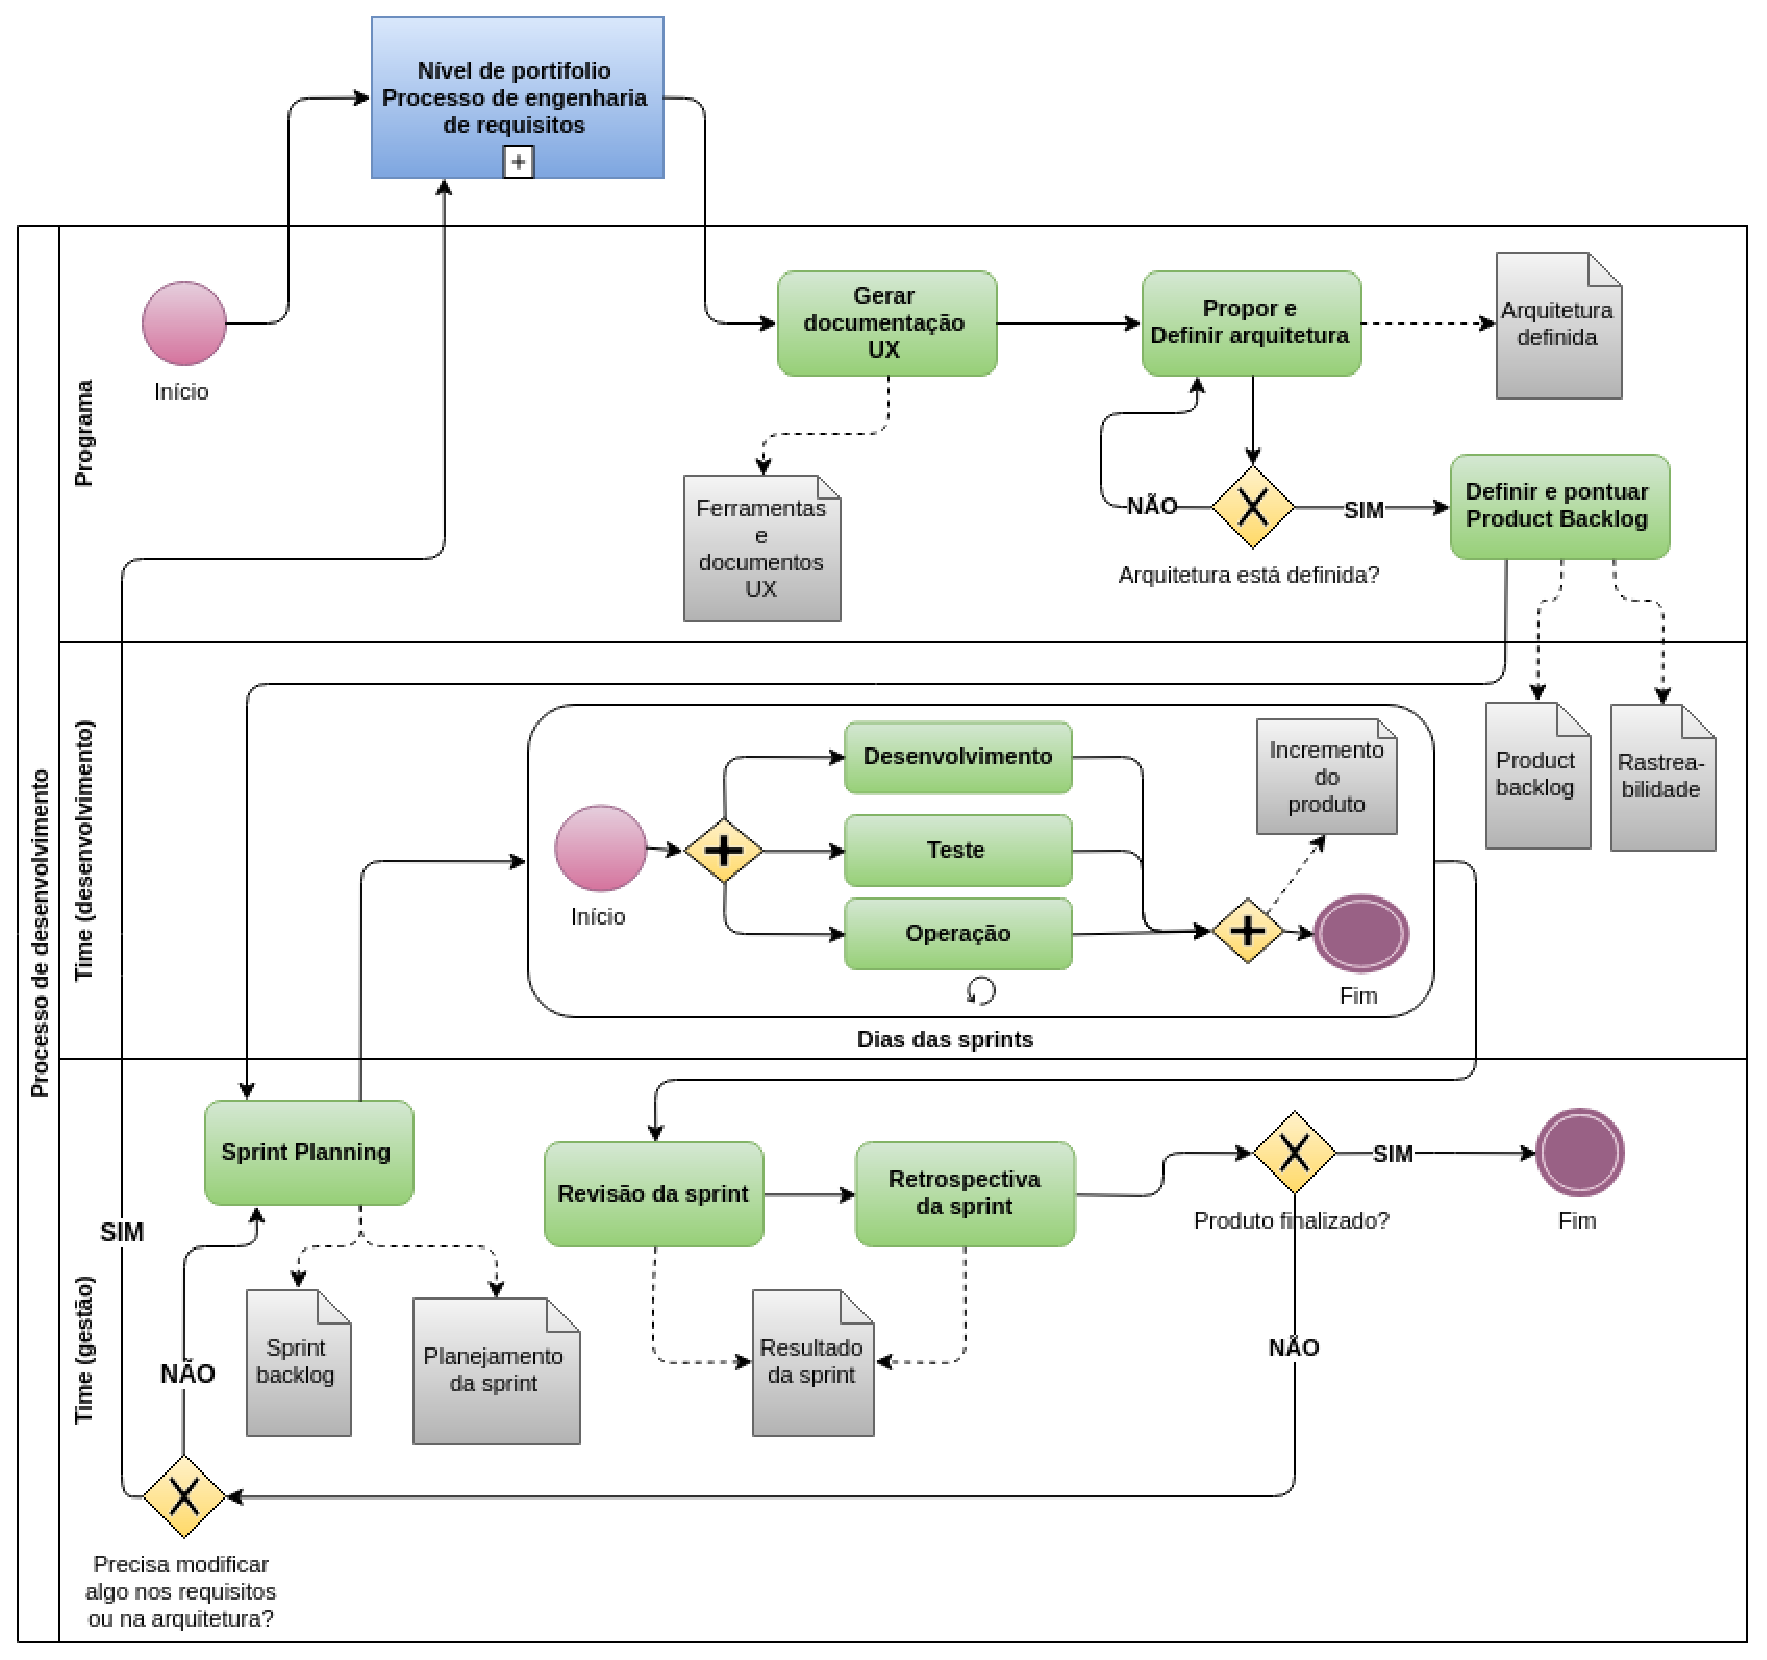
\includegraphics[keepaspectratio=true,scale=0.5]{figuras/desenvolvimento.eps}
  \caption[Processo de desenvolvimento.]{Processo de desenvolvimento. Fonte: Autor}
	\label{fig:desenvolvimento}
\end{figure}

\subsubsection{Nível de Programa}

Nível responsável pela auto-organização de times ágeis, entrega contínua de valor, criação de Features por meio dos épicos encontrados, realização de toda a documentação relacionada ao \textit{User Experience} ou UX, e definição do documento de arquitetura do software.


No nível de programa será definido a arquitetura que melhor se adapte ao projeto, utilizaremos de algumas técnicas de UX e UI para melhorar a usabilidade do software e será elaborado e pontuado as histórias de usuário do product backlog, essas serão derivadas das features definidas no nível de portfólio.

\subsubsection{Nível de Time}

Nível responsável pelo auto-gerenciamento da equipe ágil, incremento do software totalmente testado, práticas SCRUM e XP, descrição do valor por meio de User Stories e tarefas.

O nível de time se inicia com a \textit{Sprint Planning}, na qual será priorizada as histórias de usuário que serão implementadas na \textit{sprint} que se segue. Com isso inicia-se os ciclos de desenvolvimento das sprints. Dentro dessa atividade temos em paralelo o desenvolvimento, teste e operações tendo como resultado o incremento do produto.

Ao finalizar o ciclo de desenvolvimento será realizado a revisão da sprint, em que será apresentado as funcionalidades implementadas na sprint e verificar se há alguma dívida técnica para a próxima sprint que se segue. Em seguida será realizada a retrospectiva da sprint que será coletado pontos positivos, negativos e melhorias para as próximas iterações.

Todo o processo será executado de forma iterativa e incremental, ou seja, a cada iteração chamada de sprint, será retomado e avaliado se há necessidade de alguma modificação ou incremento nesses diagramas e documentos. Além de que na finalização de cada fase terá uma atividade de revisão dos documentos.
